\begin{frame}
	\myheading{Module 9.3 : Better activation functions}
\end{frame}

%%%%%%%%%%%%%%%%%%%%%%%%%%%%%%%%%%%%%%%%%%%%%%%%%%%%%%%%%%%%%%%%%%%%%%%%%%%%%%%%%%%%%%%%%

\begin{frame}
	\begin{block}{Deep Learning has evolved}
		\begin{itemize}
			\justifying
			\item \textcolor{gray}{Better optimization algorithms}
			\item \textcolor{gray}{Better regularization methods}
			\item \textcolor{red}{Better activation functions}
			\item Better weight initialization strategies
		\end{itemize}
		
	\end{block}
\end{frame}

%%%%%%%%%%%%%%%%%%%%%%%%%%%%%%%%%%%%%%%%%%%%%%%%%%%%%%%%%%%%%%%%%%%%%%%%%%%%%%%%%%%%%%%%%

\begin{frame}
	\begin{itemize}
		\justifying
		\item Before we look at activation functions, let's try to answer the following question: ``What makes Deep Neural Networks powerful ?''
	\end{itemize}
\end{frame}

%%%%%%%%%%%%%%%%%%%%%%%%%%%%%%%%%%%%%%%%%%%%%%%%%%%%%%%%%%%%%%%%%%%%%%%%%%%%%%%%%%%%%%%%%

\begin{frame}
	\begin{columns}
		
		\column{0.5\textwidth}<1->
		\begin{overlayarea}{\textwidth}{\textheight}
			\only<1-6>{
				\begin{center}
					\tikzstyle{input_neuron}=[circle,draw=red!50,fill=red!10,thick,minimum size=6mm]
\tikzstyle{hidden_neuron}=[circle,draw=blue!50,fill=cyan!10,thick,minimum size=1mm]
\tikzstyle{output_neuron}=[circle,draw=green!50,fill=green!20,thick,minimum size=1mm]
\tikzstyle{input}=[circle,draw=black!50,fill=black!20,thick,minimum size=1mm]

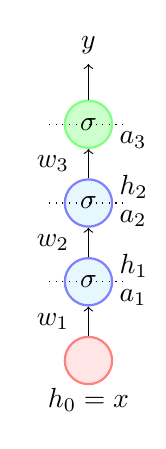
\begin{tikzpicture}

	\node [input_neuron] (neuron0) at (6,5)  {} ;
	\node (input0) at (6,4.5)  {$h_0=x$};
	\node (output0) at (6,9){$y$};
	
	\node [hidden_neuron] (neuron1) at (6,6)  {$\sigma$};
	\node [hidden_neuron] (neuron2) at (6,7)  {$\sigma$};
	\node [output_neuron] (neuron3) at (6,8)  {$\sigma$};
	
	%\draw [->] (input0) -- (neuron0);
	\draw [->] (neuron0) -- (neuron1);
	\draw [->] (neuron1) -- (neuron2);
	\draw [->] (neuron2) -- (neuron3);
	\draw [->] (neuron3) -- (output0); 
	%\draw [dotted] (5.5,5) -- (6.5,5);
	\draw [dotted] (5.5,6) -- (6.5,6);
	\draw [dotted] (5.5,7) -- (6.5,7);
	\draw [dotted] (5.5,8) -- (6.5,8);
	%\node[text width=0.01cm] at (6.4,4.8) {$a_1$};
	%\node[text width=0.01cm] at (6.4,5.2) {$h_1$};
	\node[text width=0.01cm] at (6.4,5.8) {$a_1$};
	\node[text width=0.01cm] at (6.4,6.2) {$h_1$};
	\node[text width=0.01cm] at (6.4,6.8) {$a_2$};
	\node[text width=0.01cm] at (6.4,7.2) {$h_2$};
	\node[text width=0.01cm] at (6.4,7.8) {$a_3$};
	%\node[text width=0.01cm] at (6.4,8.2) {$h_3$};
	
	\node (formula) at (5.55,5.5) {$w_1$};
	\node (formula) at (5.55,6.5) {$w_2$};
	\node (formula) at (5.55,7.5) {$w_3$};
	
\end{tikzpicture}
				\end{center}
			}
			\onslide<7->{
				\begin{figure}[H]
					%\centering
					%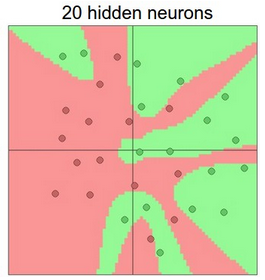
\includegraphics[width=6 cm]{images/non_linear.png}
					\includegraphics<3->[scale=0.20]{images/gaussian_3d.png}
					
					%\caption{Accuracy of sigmoid kerenel plotted against gamma, for different values of cost \textit{c}}
				\end{figure}
			}
			
		\end{overlayarea}
		
		\vspace{-.2in}
		\column{0.5\textwidth}<1->
		\begin{overlayarea}{\textwidth}{\textheight}
			%\only<1->{
				\begin{itemize}
					\justifying
					\only<1-6>{
					\onslide<1-6>{\item Consider this deep neural network }
					\onslide<2-6>{ \item Imagine if we replace the sigmoid in each layer by a simple linear transformation}
					\onslide<3-6>{
						\begin{align*}
							y=(w_{4}*(w_{3}*(w_{2}*(w_{1}x)))) \\
						\end{align*}
						
						\onslide<4-6>{\item Then we will just learn $y$ as a linear transformation of $x$}
					}
					\onslide<5-6>{\item  In other words we will be constrained to learning linear decision boundaries}
					\onslide<6>{\item  We cannot learn arbitrary decision boundaries}
					}
					\only<7->{\item  In particular, a deep linear neural network cannot learn such boundaries}
					\only<8->{\item  But a deep non linear neural network can indeed learn such boundaries (recall Universal Approximation Theorem)}
				\end{itemize}
			%}
		\end{overlayarea}
		
	\end{columns}
\end{frame}

%%%%%%%%%%%%%%%%%%%%%%%%%%%%%%%%%%%%%%%%%%%%%%%%%%%%%%%%%%%%%%%%%%%%%%%%%%%%%%%%%%%%%%%%%

\begin{frame}
	\begin{itemize}
		\justifying
		\item Now let's look at some non-linear activation functions that are typically used in deep neural networks (Much of this material is taken from Andrej Karpathy's lecture notes \footnote{http://cs231n.github.io})
	\end{itemize}
\end{frame}

%%%%%%%%%%%%%%%%%%%%%%%%%%%%%%%%%%%%%%%%%%%%%%%%%%%%%%%%%%%%%%%%%%%%%%%%%%%%%%%%%%%%%%%%%

\begin{frame}
	\begin{columns}
		\begin{column} {0.5\textwidth}
			\begin{overlayarea}{\textwidth}{\textheight}
				\begin{center}
					
					\onslide<2->{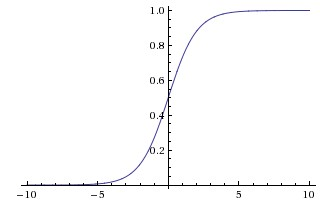
\includegraphics[scale = 0.45]{images/sigmoid.jpeg}
						
						Sigmoid
					}
				\end{center}
			\end{overlayarea}
			
		\end{column}
		\begin{column}{0.5\textwidth}
			\begin{overlayarea}{\textwidth}{\textheight}
				\begin{itemize}
					\justifying
					\item<1-> $\sigma(x) = \frac{1}{1+e^{-x}}$
					\item<2-> As is obvious, the sigmoid function compresses all its inputs to the range [0,1]
					\item<3-> Since we are always interested in gradients, let us find the gradient of this function
					\only<4->{
						\begin{align*}
							\frac{\partial \sigma(x)}{\partial x} = \sigma(x) (1- \sigma (x)) 
						\end{align*}
						\textit{(you can easily derive it)}
					}
					
					\item<5-> Let us see what happens if we use sigmoid in a deep network
				\end{itemize}
				
			\end{overlayarea}
		\end{column}
		
	\end{columns}
\end{frame}

%%%%%%%%%%%%%%%%%%%%%%%%%%%%%%%%%%%%%%%%%%%%%%%%%%%%%%%%%%%%%%%%%%%%%%%%%%%%%%%%%%%%%%%%%

\begin{frame}
	\begin{columns}
		\begin{column} {0.3\textwidth}
			\begin{center}
				\tikzstyle{input_neuron}=[circle,draw=red!50,fill=red!10,thick,minimum size=6mm]
\tikzstyle{hidden_neuron}=[circle,draw=blue!50,fill=cyan!10,thick,minimum size=1mm]
\tikzstyle{output_neuron}=[circle,draw=green!50,fill=green!20,thick,minimum size=1mm]
\tikzstyle{input}=[circle,draw=black!50,fill=black!20,thick,minimum size=1mm]

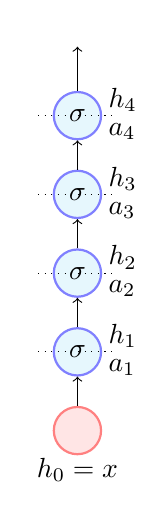
\begin{tikzpicture}

	\node [input_neuron] (neuron0) at (6,4)  {} ;
	\node (input0) at (6,3.5)  {$h_0=x$};
	\node (output0) at (6,9){};
	
	\node [hidden_neuron] (neuron1) at (6,5)  {$\sigma$};
	\node [hidden_neuron] (neuron2) at (6,6)  {$\sigma$};
	\node [hidden_neuron] (neuron3) at (6,7)  {$\sigma$};
	\node [hidden_neuron] (neuron4) at (6,8)  {$\sigma$};
	
	%\draw [->] (input0) -- (neuron0);
	\draw [->] (neuron0) -- (neuron1);
	\draw [->] (neuron1) -- (neuron2);
	\draw [->] (neuron2) -- (neuron3);
	\draw [->] (neuron3) -- (neuron4);
	\draw [->] (neuron4) -- (output0); 
	\draw [dotted] (5.5,5) -- (6.5,5);
	\draw [dotted] (5.5,6) -- (6.5,6);
	\draw [dotted] (5.5,7) -- (6.5,7);
	\draw [dotted] (5.5,8) -- (6.5,8);
	\node[text width=0.01cm] at (6.4,4.8) {$a_1$};
	\node[text width=0.01cm] at (6.4,5.2) {$h_1$};
	\node[text width=0.01cm] at (6.4,5.8) {$a_2$};
	\node[text width=0.01cm] at (6.4,6.2) {$h_2$};
	\node[text width=0.01cm] at (6.4,6.8) {$a_3$};
	\node[text width=0.01cm] at (6.4,7.2) {$h_3$};
	\node[text width=0.01cm] at (6.4,7.8) {$a_4$};
	\node[text width=0.01cm] at (6.4,8.2) {$h_4$};
	
\end{tikzpicture}
			\end{center}
		\end{column}
		\begin{column}{0.2\textwidth}
			$a_3=w_2 h_2$
			
			$h_3=\sigma(a_3)$
			
		\end{column}
		\begin{column}{0.5\textwidth}
			\begin{itemize}
				\justifying
				\item<2-> While calculating $\nabla w_{2}$ at some point in the chain rule we will encounter 
				\only<2->{
					\begin{align*}
						\frac{\partial h_{3}}{\partial a_{3}} =\frac{\partial\sigma(a_{3})}{\partial a_{3}} = \sigma(a_{3}) (1- \sigma (a_{3})) 
					\end{align*} 
				}
				
				\item<3->{What is the consequence of this ?}
				\item<4->{To answer this question let us first understand the concept of saturated neuron ?}
				
			\end{itemize}
		\end{column}
	\end{columns}
\end{frame}

%%%%%%%%%%%%%%%%%%%%%%%%%%%%%%%%%%%%%%%%%%%%%%%%%%%%%%%%%%%%%%%%%%%%%%%%%%%%%%%%%%%%%%%%%

\begin{frame}
	\begin{columns}
		\begin{column} {0.5\textwidth}
			
			\begin{center}
				\begin{tikzpicture}
	\begin{axis}[
			xmin=-2.5, xmax=2.5,
			ymin=-0.1, ymax=1.1,
			axis lines=center,
			axis on top=true,
			%domain=-2.5:2.5,
			ylabel=$y$,
			xlabel=$x$,
		]
		
		\addplot [smooth,mark=none,draw=blue,] {1/(1+exp(-2.5*\x)};
		%% Add the asymptotes
		\draw [blue, dotted, thick] (axis cs:4,+1)-- (axis cs:0,+1);
	\end{axis}
\end{tikzpicture}
			\end{center}
			\onslide<4->{\textcolor{red}{Saturated neurons thus cause the gradient to vanish.}}
			
		\end{column}
		\begin{column}{0.5\textwidth}
			\begin{itemize}
				\justifying
				\item<1-> A sigmoid neuron is said to have saturated when $\sigma(x)=1$ or $\sigma(x)=0$
				\item<2-> What would the gradient be at saturation?
				\item<3-> Well it would be 0 (you can see it from the plot or from the formula that we derived)
			\end{itemize}
			
		\end{column}
		
	\end{columns}
\end{frame}

%%%%%%%%%%%%%%%%%%%%%%%%%%%%%%%%%%%%%%%%%%%%%%%%%%%%%%%%%%%%%%%%%%%%%%%%%%%%%%%%%%%%%%%%%

\begin{frame}
	\begin{columns}
		\begin{column} {0.5\textwidth}
			\onslide<1->{\textcolor{red}{Saturated neurons thus cause the gradient to vanish.}}
			
			\begin{center}
				\tikzstyle{input_neuron}=[circle,draw=red!50,fill=orange!10,thick,minimum size=6mm]
\tikzstyle{hidden_neuron}=[circle,draw=blue!50,fill=blue!10,thick,minimum size=6mm]
\tikzstyle{output_neuron}=[circle,draw=green!50,fill=green!20,thick,minimum size=6mm]
\tikzstyle{input}=[circle,draw=black!50,fill=black!20,thick,minimum size=6mm]

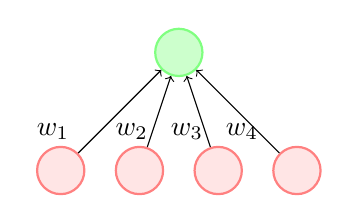
\begin{tikzpicture}

	\node [output_neuron] (out_neuron0) at (2.5,4){};
	\node [input_neuron] (input_neuron1) at (1,2.5){};
	\node [input_neuron] (input_neuron2) at (2,2.5){};
	\node [input_neuron] (input_neuron3) at (3,2.5){};
	\node [input_neuron] (input_neuron4) at (4,2.5){};
	\draw [->] (input_neuron1) -- (out_neuron0);
	\draw [->] (input_neuron2) -- (out_neuron0);
	\draw [->] (input_neuron3) -- (out_neuron0);
	\draw [->] (input_neuron4) -- (out_neuron0);
	\node[text width=0.005cm] at (0.7,3) {$w_1$};
	\node[text width=0.005cm] at (1.7,3) {$w_2$};
	\node[text width=0.005cm] at (2.4,3) {$w_3$};
	\node[text width=0.005cm] at (3.1,3) {$w_4$};
	
\end{tikzpicture}
			\end{center}
			
			\begin{center}
				$\sigma(\sum_{i=1}^{4}w_{i}x_{i})$
			\end{center}
			
			\begin{center}
				 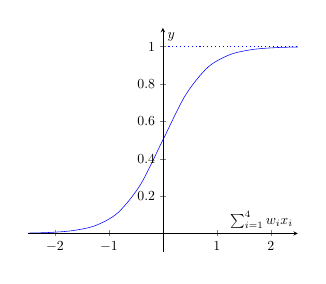
\begin{tikzpicture}[scale=0.50]
	\begin{axis}[
			xmin=-2.5, xmax=2.5,
			ymin=-0.1, ymax=1.1,
			axis lines=center,
			axis on top=true,
			%domain=-2.5:2.5,
			ylabel=$y$,
			xlabel=$\sum_{i=1}^{4} w_{i}x_{i}$,
		]
		
		\addplot [smooth,mark=none,draw=blue,] {1/(1+exp(-2.5*\x)};
		%% Add the asymptotes
		\draw [blue, dotted, thick] (axis cs:4,+1)-- (axis cs:0,+1);
	\end{axis}
\end{tikzpicture}
			\end{center}		
			
		\end{column}
		\begin{column}{0.5\textwidth}
			\begin{itemize}
				\justifying
				\item<1-> But why would the neurons saturate ?
				\item<2-> Consider what would happen if we use sigmoid neurons and initialize the weights to very high values ?
				\item<3-> The neurons will saturate very quickly
				\item<4-> The gradients will vanish and the training will stall (more on this later)	
			\end{itemize}
			
		\end{column}
		
	\end{columns}
\end{frame}

%%%%%%%%%%%%%%%%%%%%%%%%%%%%%%%%%%%%%%%%%%%%%%%%%%%%%%%%%%%%%%%%%%%%%%%%%%%%%%%%%%%%%%%%%

\begin{frame}{}
	\begin{columns}
		\column{0.5\textwidth}
		\begin{overlayarea}{\textwidth}{\textheight}
			\vspace{0.1cm}
			 
			\begin{itemize}
				\justifying
				\item Saturated neurons cause the gradient to vanish
				      \item<2-> \textcolor{red}{Sigmoids are not zero centered}
			\end{itemize}
			 
			\vspace{0.01cm}
			\begin{itemize}
				\justifying
				\vspace{0.01cm}
				\onslide<5-8>{\item Consider the gradient w.r.t. $w_1$ and $w_2$}
				\vspace{-1em}
				\onslide<5-8>
				{
					\begin{align*}
						\nabla w_1 &= \textcolor{red}{\frac{\partial{  \mathscr{L}(\textbf{w})  }}{\partial{y}} \frac{\partial{y}}{h_3} \frac{\partial{h_3}}{\partial{a_3}}} \only<5>{\textcolor{blue}{\frac{\partial{a_3}}{\partial{w_1}}}}  \hspace{0.2cm}\only<6-8>{\textcolor{cyan!100}{h_{21}}} \\
						\nabla w_2 &= \textcolor{red}{\frac{\partial{  \mathscr{L}(\textbf{w})  }}{\partial{y}} \frac{\partial{y}}{h_3} \frac{\partial{h_3}}{\partial{a_3}}} \only<5>{\textcolor{blue}{\frac{\partial{a_3}}{\partial{w_2}}}}  \hspace{0.2cm}\only<6-8>{\textcolor{cyan!100}{h_{22}}}
						% \textcolor{red}{\frac{\partial{h}}{\partial{y}} \frac{\partial{y}}{h_3} \frac{\partial{h_3}}{\partial{a_3}}} \only<5>{\textcolor{blue}{\frac{\partial{a_3}}{\partial{w_3}}}}  \hspace{0.2cm}\only<6-8>{\textcolor{cyan!100}{h_{23}}}
					\end{align*}
					   
				}
				
				\onslide<6-8>{\item Note that $\textcolor{cyan!100}{h_{21}}$ and $\textcolor{cyan!100}{h_{22}}$ are between $[0,1]$ (\textit{i.e.}, they are both positive)}
				\onslide<7-8>{\item So if the first common term (in red) is positive (negative) then both $\nabla w_1$ and $\nabla w_2$ are positive (negative)}
				%\onslide<8-9>{\item And if the first common term (in red) is negative then both $\nabla w_1$ and $\nabla w_2$ are negative}
				
				 
			\end{itemize}
			 
		\end{overlayarea}
		\column{0.5\textwidth}
		\begin{overlayarea}{\textwidth}{\textheight}
			 
			\vspace{0.1cm}
			\onslide<3-8>{\begin{itemize}
				\justifying
				\item Why is this a problem??
				\end{itemize}}
			
			\vspace{-0.2in}
			
			\begin{center}
				\only<4-8>{
					\tikzstyle{input_neuron}=[circle,draw=red!50,fill=red!10,thick,minimum size=6mm]
\tikzstyle{hidden_neuron}=[circle,draw=blue!50,fill=cyan!10,thick,minimum size=6mm]
\tikzstyle{output_neuron}=[circle,draw=green!50,fill=green!10,thick,minimum size=6mm]
\tikzstyle{input}=[circle,draw=black!50,fill=black!20,thick,minimum size=6mm]

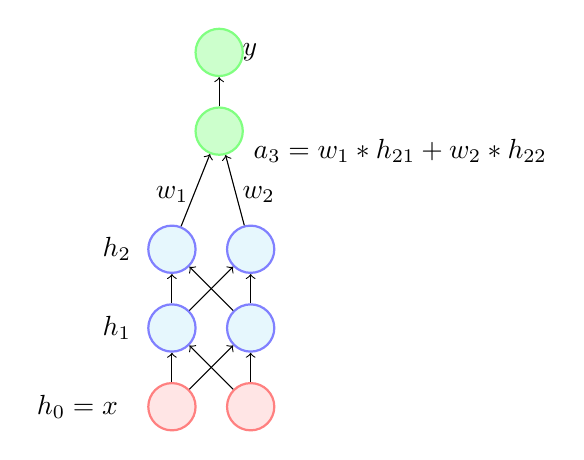
\begin{tikzpicture}
	
	\node [input_neuron] (neuron01) at (7,6.5){} ;
	\node [input_neuron] (neuron02) at (8,6.5){};
	\node[text width=0.005cm] at (6.8,9.2) {$w_1$};
	\node[text width=0.005cm] at (7.9,9.2) {$w_2$};
	%\node[text width=0.005cm] at (7.9,10.25) {$h_3$};
	\node  at (9.9,9.75) {$a_3 = w_1*h_{21} + w_2 * h_{22}$};
	\node[text width=0.005cm] at (7.9,11.0) {$y$};
	%\node at (9.9,11.5) {$a_3 = w_1*h_{21} + w_2 * h_{22})$};
	
	
	\node (hidden1) at (5.8,6.5){$h_0=x$};
	\node (hidden2) at (6.3,7.5){$h_1$};
	\node (hidden3) at (6.3,8.5){$h_2$};
	%\node(input0) at(7.6,5.8){$h_o = x$};
	%\node(text) at (10,9.3){All outputs are between [0,1]};
	\node [hidden_neuron] (neuron11) at (7,7.5){}  ;
	\node [hidden_neuron] (neuron12) at (8,7.5) {} ;
	%\node [hidden_neuron] (neuron13) at (9,7.5)  ;
	
	\node [hidden_neuron] (neuron21) at (7,8.5){}  ;
	\node [hidden_neuron] (neuron22) at (8,8.5) {} ;
	%\node [hidden_neuron] (neuron23) at (9,8.5)  ;
	
	\node [output_neuron] (neuron42) at (7.6,10.0) {} ;
	\node [output_neuron] (neuron52) at (7.6,11.0) {} ;
	%\draw[->,red](text)--(neuron02);
	%\draw[->,red](text)--(neuron12);
	%\draw[->,red](text)--(neuron22);
	
	\draw[->](neuron01)--(neuron11);
	\draw[->](neuron01)--(neuron12);
	%\draw[->](neuron01)--(neuron13);
	
	\draw[->](neuron02)--(neuron11);
	\draw[->](neuron02)--(neuron12);
	%\draw[->](neuron02)--(neuron13);
	
	%\draw[->](neuron03)--(neuron11);
	%\draw[->](neuron03)--(neuron12);
	%\draw[->](neuron03)--(neuron13);
	
	\draw[->](neuron11)--(neuron21);
	\draw[->](neuron12)--(neuron21);
	%\draw[->](neuron13)--(neuron21);
	
	\draw[->](neuron11)--(neuron22);
	\draw[->](neuron12)--(neuron22);
	%\draw[->](neuron13)--(neuron22);
	
	%\draw[->](neuron11)--(neuron23);
	%\draw[->](neuron12)--(neuron23);
	%\draw[->](neuron13)--(neuron23);
	
	\draw[->](neuron21)--(neuron42);
	\draw[->](neuron22)--(neuron42);
	%\draw[->](neuron23)--(neuron42);
	\draw[->](neuron42)--(neuron52);
	%\node (output1) at (8,10.5){};
	%\node (output0) at (7,10.5){$y_1$};
	
	%\node (output2) at (9,10.5){$y_3$};
	
\end{tikzpicture}
				}
			\end{center}		
			
			%%error free from here
			\vspace{-0.2in}
			\begin{itemize}
				\justifying
				\onslide<8>{\item Essentially, either all the gradients at a layer are positive or all the gradients at a layer are negative}
				% Same holds for gradients at layers $h_2$ and $h_1$ also
			\end{itemize}
		\end{overlayarea}
		
		
		
	\end{columns}
\end{frame}

%%%%%%%%%%%%%%%%%%%%%%%%%%%%%%%%%%%%%%%%%%%%%%%%%%%%%%%%%%%%%%%%%%%%%%%%%%%%%%%%%%%%%%%%%

\begin{frame}{}
	\begin{columns}
		\column{0.5\textwidth}
		\begin{overlayarea}{\textwidth}{ \textheight}
			\vspace{0.1cm}
			\begin{itemize}
				\justifying
				\item Saturated neurons cause the gradient to vanish
				\item \textcolor{red}{Sigmoids are not zero centered}
			\end{itemize}
		\end{overlayarea}
		 
		\column{0.5\textwidth}
		\begin{overlayarea}{\textwidth}{\textheight}
			\vspace{0.1cm}
			\begin{itemize}
				\justifying
				\item This restricts the possible update directions
			\end{itemize}
			   
			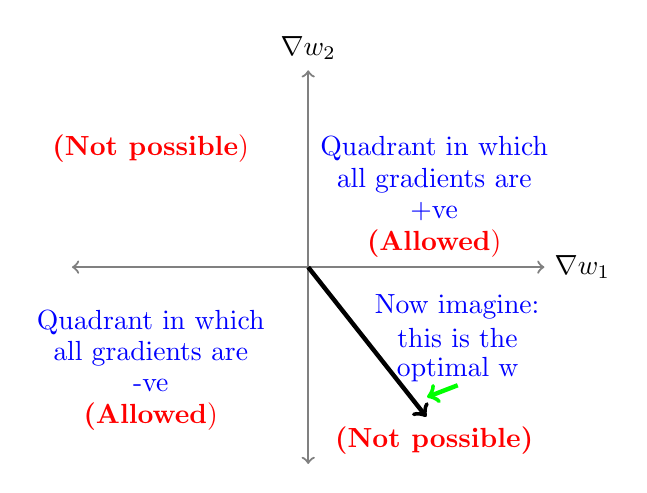
\begin{tikzpicture}

	\onslide<1-3>{
		\draw [thick, gray, <->] (10,2) -- (10,7)      % draw y-axis line
		node [above, black] {$\nabla w_2$};              % add label for y-axis
		%node [below,black]{$-y$};
		\draw [thick, gray, <->] (7,4.5) -- (13,4.5)      % draw x-axis line
		node [right, black] {$\nabla w_1$};              % add label for x-axis
	}


	\onslide<2-3>{\node[blue](text) at (8,6){\textcolor{red}{\textbf{(Not possible})}};}
	\onslide<2-3>{\node[blue](text) at (11.6,6){Quadrant in which};}
	\onslide<2-3>{\node[blue](text) at (11.6,5.6){all gradients are};}
	\onslide<2-3>{\node[blue](text) at (11.6,5.2){+ve};}
	\onslide<2-3>{\node[blue](text) at (11.6,4.8){\textcolor{red}{\textbf{(Allowed})}};}

	\onslide<2-3>{\node[blue](text) at (8,3.8){Quadrant in which};}
	\onslide<2-3>{\node[blue](text) at (8,3.4){all gradients are};}
	\onslide<2-3>{\node[blue](text) at (8,3){-ve};}
	\onslide<2-3>{\node[blue](text) at (8,2.6){\textcolor{red}{\textbf{(Allowed})}};}
	\onslide<2-3>{\node[blue](text) at (11.6,2.3){\textcolor{red}{\textbf{(Not possible)}}};}

	\onslide<3>{
		\draw[->,draw=black,ultra thick](10,4.5)--(11.5,2.6);
		\draw[->,draw=green,ultra thick](11.899,3.0)--(11.51,2.85);
	}
	\onslide<3>{
		\node(textmarked1) at (11.892,4){\textcolor{blue}{Now imagine:}};
		\node(textmarked2) at (11.896,3.6){\textcolor{blue}{this is the}};
		\node(textmarked3) at (11.899,3.2){\textcolor{blue}{optimal w}};

	}
	
\end{tikzpicture} 
		\end{overlayarea}
	\end{columns}
\end{frame}

%%%%%%%%%%%%%%%%%%%%%%%%%%%%%%%%%%%%%%%%%%%%%%%%%%%%%%%%%%%%%%%%%%%%%%%%%%%%%%%%%%%%%%%%%

\begin{frame}
	\begin{columns}
		\column{0.5\textwidth}
		\begin{overlayarea}{\textwidth}{\textheight}
			\vspace{0.1cm}
			\begin{itemize}
				\justifying
				\item Saturated neurons cause the gradient to vanish
				\item \textcolor<1-7>{red}{Sigmoids are not zero centered}
				      \only<8>{\item \textcolor{red}{And lastly, sigmoids are computationally expensive (because of \begin{math}\exp{(x)}\end{math})}}
			\end{itemize}
		\end{overlayarea}
		\column{0.5\textwidth}
		\begin{overlayarea}{\textwidth}{\textheight}
			\vspace{1cm}
  			\begin{tikzpicture}

	\draw [thick, gray, <->] (10,2) -- (10,7)      % draw y-axis line
	node [above, black] {$\nabla w_2$};              % add label for y-axis
	%node [below,black]{$-y$};
	\draw [thick, gray, <->] (7,4.5) -- (13,4.5)      % draw x-axis line
	node [right, black] {$\nabla w_1$};  
	\draw[->,draw=black,ultra thick](10,4.5)--(11.5,2.6);
	\only<2-8>{
		\draw[->,draw=green!100,thick](10,4.5) -- (10.6,5.3);}
	\only<3-8>{
		\draw[->,draw=blue,thick](10.6,5.3)--(10.6,4.5);}
	\only<4-8>{
		\draw[->,draw=red,thick](10.6,4.5)--(11,4.5);}
	\only<5-8>{
		\draw[->,draw=blue,thick](11,4.5)--(11,3.8);}
	\only<6-8>{
		\draw[->,draw=red,thick](11,3.8)--(11.5,3.8);}
	\only<2-8>{
		\node(label1) at (11.5,6.6){starting from this};
		\node(label2) at (11.9,6.2){initial position};
		\node(label3) at (12.3,5.8){only way to reach it};
		\node(label4) at (12.6,5.4){is by taking a \textcolor{red}{zigzag} path};
		\draw[->,draw=black,thick](10.5,6.45)--(10.5,5.35);
	}
	
	\only<7-8>{    \draw[->,draw=blue,thick](11.5,3.8)--(11.5,2.6);}
	
\end{tikzpicture}      
		\end{overlayarea}
		  
	\end{columns}
\end{frame}

%%%%%%%%%%%%%%%%%%%%%%%%%%%%%%%%%%%%%%%%%%%%%%%%%%%%%%%%%%%%%%%%%%%%%%%%%%%%%%%%%%%%%%%%%

\begin{frame}
	\begin{columns}
		\column {0.5\textwidth}
		tanh(x)
		\begin{center}
			\begin{tikzpicture}

	\begin{axis}[
			%xmin=-2.5, xmax=2.5,
			%ymin=-1.5, ymax=1.5,
			axis lines=center,
			axis on top=true,
			%domain=-2.5:2.5,
			ylabel=$y$,
			xlabel=$x$,
		]
		
		\addplot [smooth,mark=none,draw=blue,] {tanh(\x)};
		%% Add the asymptotes
		\draw [blue, dotted, thick] (axis cs:-2.5,-1)-- (axis cs:0,-1);
		\draw [blue, dotted, thick] (axis cs:+2.5,+1)-- (axis cs:0,+1);
		\node(text) at (axis cs:0.2,-0.1) {0};
	\end{axis}
	
\end{tikzpicture}
		\end{center}
		
		\begin{center}
			f(x) = tanh(x)
		\end{center}
				
		%\end{column}
		\column{0.5\textwidth}
		\begin{overlayarea}{\textwidth}{\textheight}
			
			\begin{itemize}
				\justifying
				\item<1-> Compresses all its inputs to the range [-1,1]
				\item<2-> \textcolor{green}{Zero centered} 
				\item<3-> What is the derivative of this function?
				\onslide<4->{
					\begin{align*}
						\frac{\partial tanh(x)}{\partial x} = (1 - tanh^{2}(x)) 
					\end{align*}  
				}
				\item<5-> \textcolor{red}{The gradient still vanishes at saturation}
				\item<6-> \textcolor{red}{Also computationally expensive}
			\end{itemize}
		\end{overlayarea}
		%\end{column}
		
	\end{columns}
	
\end{frame}

%%%%%%%%%%%%%%%%%%%%%%%%%%%%%%%%%%%%%%%%%%%%%%%%%%%%%%%%%%%%%%%%%%%%%%%%%%%%%%%%%%%%%%%%%

\begin{frame}
	\begin{columns}
		\begin{column} {0.5\textwidth}
			ReLU
			\begin{center}
				
				\begin{figure}
					\includegraphics<1-2>[scale=0.2]{images/relu_1.png}
					\includegraphics<3->[scale=0.2]{images/relu_sigm.png}
				\end{figure}
				
			\end{center}
			
			\begin{center}
				\onslide<1-2>{
					\begin{math}
						f(x) = max(0,x)
					\end{math}
				}
				\onslide<3->{
					\begin{math}
						f(x) = max(0,x+1) - max(0, x-1)
					\end{math}
				}
			\end{center}
			
			
		\end{column}
		\begin{column}{0.5\textwidth}
			\begin{itemize}
				\justifying
				\item<1-> Is this a non-linear function?
				\item<2-> Indeed it is!
				\item<3-> In fact we can combine two ReLU units to recover a piecewise linear approximation of the sigmoid function
			\end{itemize}
			
		\end{column}
		
	\end{columns}
	
	    
\end{frame}

%%%%%%%%%%%%%%%%%%%%%%%%%%%%%%%%%%%%%%%%%%%%%%%%%%%%%%%%%%%%%%%%%%%%%%%%%%%%%%%%%%%%%%%%%

\begin{frame}
	\begin{columns}
		\begin{column} {0.5\textwidth}
			ReLU
			
			\begin{center}
				\begin{figure}
					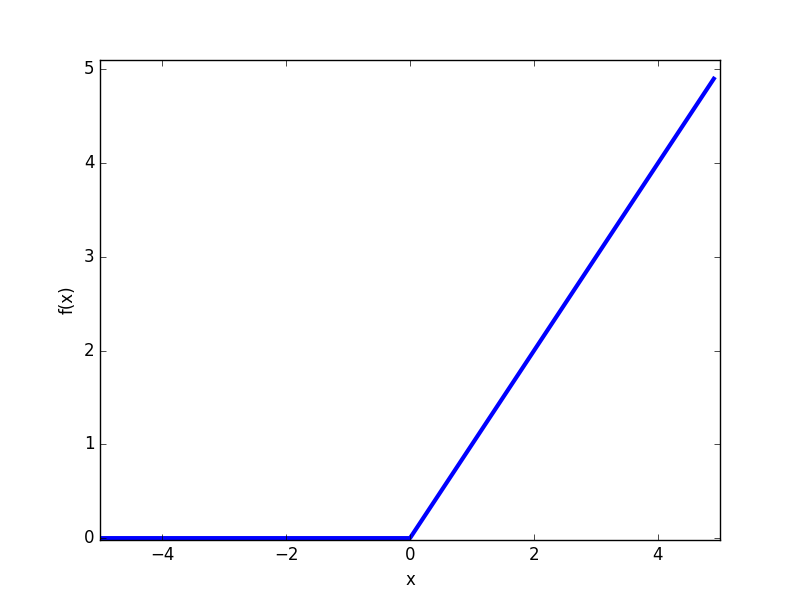
\includegraphics[scale=0.2]{images/relu_1.png}
				\end{figure}
			\end{center}
			\begin{center}
				\begin{math}
					f(x) = max(0,x)
				\end{math}
				
			\end{center}
			
		\end{column}
		\begin{column}{0.5\textwidth}
			Advantages of ReLU
			\begin{itemize}
				\justifying
				\item<1-> Does not saturate in the positive region
				\item<2-> Computationally efficient
				\item<3-> In practice converges much faster than $sigmoid/tanh^1$ 
			\end{itemize}
			
		\end{column}
		
	\end{columns}
	\footnotetext[1]{ImageNet Classification with Deep Convolutional Neural Networks- Alex Krizhevsky
	Ilya Sutskever, Geoffrey E. Hinton, 2012}
	    
\end{frame}

%%%%%%%%%%%%%%%%%%%%%%%%%%%%%%%%%%%%%%%%%%%%%%%%%%%%%%%%%%%%%%%%%%%%%%%%%%%%%%%%%%%%%%%%%

\begin{frame}
	\begin{columns}
		\begin{column} {0.4\textwidth}
			\begin{center}
				\tikzstyle{input_neuron}=[circle,draw=red!50,fill=red!10,thick,minimum size=6mm]
\tikzstyle{hidden_neuron}=[circle,draw=blue!50,fill=cyan!10,thick,minimum size=6mm]
\tikzstyle{output_neuron}=[circle,draw=green!50,fill=green!20,thick,minimum size=6mm]
\tikzstyle{input}=[circle,draw=black!50,fill=black!20,thick,minimum size=6mm]

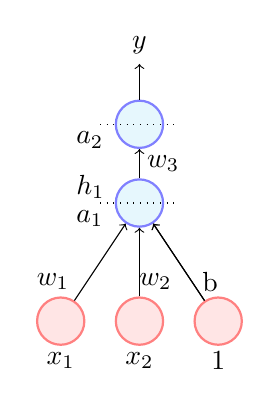
\begin{tikzpicture}

	\node (input1) at (1,2)  {$x_{1}$};
	\node (input2) at (2,2)  {$x_{2}$};
	\node (input3) at (3,2)  {$1$};
	\node (output) at (2,6)  {$y$};
	
	\node [hidden_neuron] (hidden_neuron2) at (2,5) {};
	\node [hidden_neuron] (hidden_neuron1) at (2,4)  {} ;
	\node [input_neuron] (input_neuron1) at (1,2.5) {};
	\node [input_neuron] (input_neuron2) at (2,2.5) {};
	\node [input_neuron] (input_neuron3) at (3,2.5) {};
	\draw [->] (input_neuron1) -- (hidden_neuron1);
	\draw [->] (input_neuron2) -- (hidden_neuron1);
	\draw [->] (input_neuron3) -- (hidden_neuron1);
	\draw [->] (input_neuron3) -- (hidden_neuron1);
	\draw [->] (hidden_neuron1) -- (hidden_neuron2);
	\draw [->] (hidden_neuron2) -- (output);
	
	\draw [dotted] (1.5,5) -- (2.5,5);
	\draw [dotted] (1.5,4) -- (2.5,4);
	\node[text width=0.005cm] at (0.7,3) {$w_1$};
	\node[text width=0.005cm] at (2,3) {$w_2$};
	\node[text width=0.005cm] at (2.8,3) {b};
	\node[text width=0.005cm] at (1.2,4.2) {$h_1$};
	\node[text width=0.005cm] at (1.2,3.8) {$a_1$};
	%\node[text width=0.005cm] at (1.2,5.2) {$h_2$};
	\node[text width=0.005cm] at (1.2,4.8) {$a_2$};
	
	\node[text width=0.005cm] at (2.1,4.5) {$w_3$};
	
\end{tikzpicture}
			\end{center}
		\end{column}
		\begin{column}{0.6\textwidth}
			\begin{itemize}
				\justifying
				\item<1-> In practice there is a caveat
				\item<2-> Let's see what is the derivative of ReLU(x)\\
				%\begin{comment}
				\begin{align*}
					\frac{\partial ReLU(x)}{\partial x} & = 0 \quad {if \quad x < 0} \\
					                                    & = 1 \quad {if \quad x > 0} 
				\end{align*}
				
				%\end{comment}  

				\item<3-> Now consider the given network 
				\item<4-> What would happen if at some point a large gradient causes the bias $b$ to be updated to a large negative value?
			\end{itemize}
			
		\end{column}
		
	\end{columns}
\end{frame}

%%%%%%%%%%%%%%%%%%%%%%%%%%%%%%%%%%%%%%%%%%%%%%%%%%%%%%%%%%%%%%%%%%%%%%%%%%%%%%%%%%%%%%%%%

\begin{frame}
	\begin{columns}
		
		\begin{column} {0.4\textwidth}
			\begin{center}
				\tikzstyle{input_neuron}=[circle,draw=red!50,fill=red!10,thick,minimum size=6mm]
\tikzstyle{hidden_neuron}=[circle,draw=blue!50,fill=cyan!10,thick,minimum size=6mm]
\tikzstyle{output_neuron}=[circle,draw=green!50,fill=green!20,thick,minimum size=6mm]
\tikzstyle{input}=[circle,draw=black!50,fill=black!20,thick,minimum size=6mm]

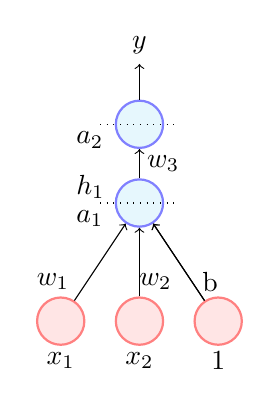
\begin{tikzpicture}

	\node (input1) at (1,2)  {$x_{1}$};
	\node (input2) at (2,2)  {$x_{2}$};
	\node (input3) at (3,2)  {$1$};
	\node (output) at (2,6)  {$y$};
	
	\node [hidden_neuron] (hidden_neuron2) at (2,5) {};
	\node [hidden_neuron] (hidden_neuron1) at (2,4)  {} ;
	\node [input_neuron] (input_neuron1) at (1,2.5) {};
	\node [input_neuron] (input_neuron2) at (2,2.5) {};
	\node [input_neuron] (input_neuron3) at (3,2.5) {};
	\draw [->] (input_neuron1) -- (hidden_neuron1);
	\draw [->] (input_neuron2) -- (hidden_neuron1);
	\draw [->] (input_neuron3) -- (hidden_neuron1);
	\draw [->] (input_neuron3) -- (hidden_neuron1);
	\draw [->] (hidden_neuron1) -- (hidden_neuron2);
	\draw [->] (hidden_neuron2) -- (output);
	
	\draw [dotted] (1.5,5) -- (2.5,5);
	\draw [dotted] (1.5,4) -- (2.5,4);
	\node[text width=0.005cm] at (0.7,3) {$w_1$};
	\node[text width=0.005cm] at (2,3) {$w_2$};
	\node[text width=0.005cm] at (2.8,3) {b};
	\node[text width=0.005cm] at (1.2,4.2) {$h_1$};
	\node[text width=0.005cm] at (1.2,3.8) {$a_1$};
	%\node[text width=0.005cm] at (1.2,5.2) {$h_2$};
	\node[text width=0.005cm] at (1.2,4.8) {$a_2$};
	
	\node[text width=0.005cm] at (2.1,4.5) {$w_3$};
	
\end{tikzpicture}
			\end{center}
		\end{column}
		
		\begin{column}{0.6\textwidth}
			\vspace{-0.2in}
			
			\begin{align*}
				w_{1}x_{1} +w_{2}x_{2} + b < 0 \quad [if \quad b<<0]
			\end{align*}
			\vspace{-0.2in}
			
			\begin{itemize}
				\justifying
				\item<1-> The neuron would output 0 [dead neuron]
				\item<2-> Not only would the output be 0 but during backpropagation even the gradient $\frac{\partial h_{1}}{\partial a_{1}}$ would be zero
				\item<3-> The weights $w_{1}$, $w_{2}$ and b will not get updated [$\because$ there will be a zero term in the chain rule]
				
				\begin{align*}
					\nabla w_1 =\frac{\partial\mathscr{L}(\theta)}{\partial y}.\frac{\partial y}{\partial a_{2}}.\frac{\partial a_{2}}{\partial h_{1}}.\frac{\partial h_{1}}{\partial a_{1}}.\frac{\partial a_{1}}{\partial w_{1}}
				\end{align*}
				
				\item<4-> The neuron will now stay dead forever!!
			\end{itemize}
			
		\end{column}
		
	\end{columns}
\end{frame}

%%%%%%%%%%%%%%%%%%%%%%%%%%%%%%%%%%%%%%%%%%%%%%%%%%%%%%%%%%%%%%%%%%%%%%%%%%%%%%%%%%%%%%%%%

\begin{frame}
	\begin{columns}
		\begin{column} {0.5\textwidth}
			\begin{center}
				\tikzstyle{input_neuron}=[circle,draw=red!50,fill=red!10,thick,minimum size=6mm]
\tikzstyle{hidden_neuron}=[circle,draw=blue!50,fill=cyan!10,thick,minimum size=6mm]
\tikzstyle{output_neuron}=[circle,draw=green!50,fill=green!20,thick,minimum size=6mm]
\tikzstyle{input}=[circle,draw=black!50,fill=black!20,thick,minimum size=6mm]

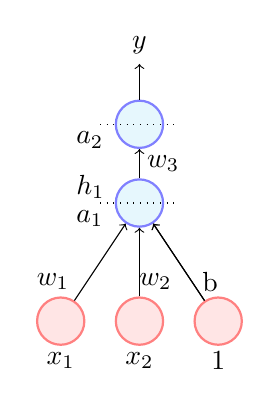
\begin{tikzpicture}

	\node (input1) at (1,2)  {$x_{1}$};
	\node (input2) at (2,2)  {$x_{2}$};
	\node (input3) at (3,2)  {$1$};
	\node (output) at (2,6)  {$y$};
	
	\node [hidden_neuron] (hidden_neuron2) at (2,5) {};
	\node [hidden_neuron] (hidden_neuron1) at (2,4)  {} ;
	\node [input_neuron] (input_neuron1) at (1,2.5) {};
	\node [input_neuron] (input_neuron2) at (2,2.5) {};
	\node [input_neuron] (input_neuron3) at (3,2.5) {};
	\draw [->] (input_neuron1) -- (hidden_neuron1);
	\draw [->] (input_neuron2) -- (hidden_neuron1);
	\draw [->] (input_neuron3) -- (hidden_neuron1);
	\draw [->] (input_neuron3) -- (hidden_neuron1);
	\draw [->] (hidden_neuron1) -- (hidden_neuron2);
	\draw [->] (hidden_neuron2) -- (output);
	
	\draw [dotted] (1.5,5) -- (2.5,5);
	\draw [dotted] (1.5,4) -- (2.5,4);
	\node[text width=0.005cm] at (0.7,3) {$w_1$};
	\node[text width=0.005cm] at (2,3) {$w_2$};
	\node[text width=0.005cm] at (2.8,3) {b};
	\node[text width=0.005cm] at (1.2,4.2) {$h_1$};
	\node[text width=0.005cm] at (1.2,3.8) {$a_1$};
	%\node[text width=0.005cm] at (1.2,5.2) {$h_2$};
	\node[text width=0.005cm] at (1.2,4.8) {$a_2$};
	
	\node[text width=0.005cm] at (2.1,4.5) {$w_3$};
	
\end{tikzpicture}
			\end{center}
				
		\end{column}
		\begin{column}{0.5\textwidth}
			\begin{itemize}
				\justifying
				\item<1-> In practice a large fraction of ReLU units can die if the learning rate is set too high
				\item<2-> It is advised to initialize the bias to a positive value (0.01)
				\item<3-> Use other variants of ReLU (as we will soon see)
			\end{itemize}
			
		\end{column}
		
	\end{columns}
\end{frame}

%%%%%%%%%%%%%%%%%%%%%%%%%%%%%%%%%%%%%%%%%%%%%%%%%%%%%%%%%%%%%%%%%%%%%%%%%%%%%%%%%%%%%%%%%

\begin{frame}
	\begin{columns}
		\begin{column} {0.5\textwidth}
			Leaky ReLU
			\begin{center}
				\begin{tikzpicture}

	\draw[->] (-2,0) -- (2,0) node[right] {x};
	\draw[->] (0,-2) -- (0,2) node[above] {y};
	\draw[scale=0.5,domain=-3:3,smooth,variable=\x,blue] plot ({\x},{max(0.1*\x,\x});

\end{tikzpicture}
			\end{center}
			
			\begin{center}
				f(x) = max(0.01x,x)
			\end{center}
			
		\end{column}
		\begin{column}{0.5\textwidth}
			\begin{itemize}
				\justifying
				\item<1-> No saturation
				\item<2-> Will not die ($0.01 x$ ensures that at least a small gradient will flow through)
				\item<3-> Computationally efficient
				\item<4-> Close to zero centered ouputs
			\end{itemize}
			
			\onslide<5->{
				\begin{align*}
					\textbf{Parametric ReLU}                                      \\
					f(x) = \max(\alpha x , x)                                     \\
					\alpha \quad \textit{is a parameter of the model}             \\
					\alpha \quad \textit{will get updated during backpropagation} \\
				\end{align*}
			}
		\end{column}
		
	\end{columns}    
\end{frame}

%%%%%%%%%%%%%%%%%%%%%%%%%%%%%%%%%%%%%%%%%%%%%%%%%%%%%%%%%%%%%%%%%%%%%%%%%%%%%%%%%%%%%%%%%

\begin{frame}
\begin{flushleft}
Exponential Linear Unit
\end{flushleft}
	
	\begin{columns}
		\begin{column} {0.5\textwidth}
			\begin{center}
				\begin{tikzpicture}

	\draw[->] (-2,0) -- (2,0) node[right] {x};
	\draw[->] (0,-2) -- (0,2) node[above] {y};
	\draw[scale=0.5,domain=0:3,smooth,variable=\x,blue] plot ({\x},{\x});
	\draw[scale=0.5,domain=-3:0,smooth,variable=\x,blue] plot ({\x},{exp(\x)-1});

\end{tikzpicture}
			\end{center}
			
			\begin{align*}
				f(x) & = x \quad {if \quad x > 0}           \\
				     & = a e^{x} - 1 \quad {if \quad x \leq 0} 
			\end{align*}
			
		\end{column}
		\begin{column}{0.5\textwidth}
			\begin{itemize}
				\justifying
				\item<1-> All benefits of ReLU
				\item<2-> $a e^{x} - 1$ ensures that at least a small gradient will flow through 
				\item<3-> Close to zero centered outputs
				\item<4-> Expensive (requires computation of exp(x))
			\end{itemize}
			
		\end{column}
		
	\end{columns}    
\end{frame}

%%%%%%%%%%%%%%%%%%%%%%%%%%%%%%%%%%%%%%%%%%%%%%%%%%%%%%%%%%%%%%%%%%%%%%%%%%%%%%%%%%%%%%%%%

\begin{frame}
\begin{flushleft}
Maxout Neuron
\end{flushleft}
	
	\begin{columns}
		\begin{column} {0.5\textwidth}
			
			
			\begin{equation*}
				max (w_1^T x + b_1, w_2^T x+b_2)
			\end{equation*}
			
			
		\end{column}
		\begin{column}{0.5\textwidth}
			\begin{itemize}
				\justifying
				\item<1-> Generalizes ReLU and Leaky ReLU
				\item<2-> No saturation! No death!
				\item<3-> \textcolor{red}{Doubles the number of parameters}
			\end{itemize}
			
		\end{column}
		
	\end{columns}    
\end{frame}

%%%%%%%%%%%%%%%%%%%%%%%%%%%%%%%%%%%%%%%%%%%%%%%%%%%%%%%%%%%%%%%%%%%%%%%%%%%%%%%%%%%%%%%%%

\begin{frame}
	\begin{block}{Things to Remember}
		\begin{itemize}[<+->]
			\justifying
			\item Sigmoids are bad 
			\item ReLU is more or less the standard unit for Convolutional Neural Networks
			\item Can explore Leaky ReLU/Maxout/ELU 
			\item tanh sigmoids are still used in LSTMs/RNNs (we will see more on this later)          
		\end{itemize}
		
	\end{block}
\end{frame}